\documentclass[xcolor=x11names,compress]{beamer}

\usepackage{graphicx}
\usepackage{epstopdf}
\usepackage{tikz}
\usepackage{caption}
\usepackage{subcaption}
\captionsetup{compatibility=false}
\usepackage[polish]{babel}
\usepackage[utf8]{inputenc}
\usepackage[T1]{fontenc}
\usetikzlibrary{decorations.fractals}

%% Beamer Layout %%%%%%%%%%%%%%%%%%%%%%%%%%%%%%%%%%
%%  This Beamer template was created by Cameron Bracken.
%%  Anyone can freely use or modify it for any purpose
%%  without attribution.
%%
%%  Last Modified: January 9, 2009
\useoutertheme[subsection=false,shadow]{miniframes}
\useinnertheme{default}
\usefonttheme{serif}
\usepackage{palatino}



\setbeamerfont{title like}{shape=\scshape}
\setbeamerfont{frametitle}{shape=\scshape}

\setbeamercolor*{lower separation line head}{bg=DeepSkyBlue4} 
\setbeamercolor*{normal text}{fg=black,bg=white} 
\setbeamercolor*{alerted text}{fg=red} 
\setbeamercolor*{example text}{fg=black} 
\setbeamercolor*{structure}{fg=black} 
 
\setbeamercolor*{palette tertiary}{fg=black,bg=black!10} 
\setbeamercolor*{palette quaternary}{fg=black,bg=black!10} 

\setbeameroption{show notes}

\renewcommand{\(}{\begin{columns}}
\renewcommand{\)}{\end{columns}}
\newcommand{\<}[1]{\begin{column}{#1}}
\renewcommand{\>}{\end{column}}
%%%%%%%%%%%%%%%%%%%%%%%%%%%%%%%%%%%%%%%%%%%%%%%%%%

\begin{document}

%\section{\scshape Spis treści}
\begin{frame}
\title{Metody nieparametryczne}
%\subtitle{SUBTITLE}
\author{
	Bartłomiej Miga\\
	Jakub Rakoczy\\
	Wojciech Padykuła
}
\date{
	\begin{tikzpicture}[decoration=Koch curve type 2] 
		\draw[DeepSkyBlue4] decorate{ decorate{ decorate{ (0,0) -- (3,0) }}}; 
	\end{tikzpicture}  
	\\
	\vspace{1cm}
	\today
}
\titlepage
\end{frame}

\begin{frame}
\tableofcontents
\end{frame}

\section{\scshape M. Nieparametryczne}

\subsection{Wstęp}
\begin{frame}{Wady i zalety metod parametrycznych}
	\note{W idealnym dla naukowca świecie badane przez niego wartości podlegają dokładnie jednemu z typowych rozkładów matematycznych, który jest z góry znany. Niestety w praktyce rozkład trzeba zgadywać, a dane z reguły i tak nie będą do niego idealnie pasować. Rzeczywiste rozkłady są z reguły dużo bardziej złożone, ponieważ składa się na nie wiele czynników, a rozkłady teoretyczne pozwalają uwzględnić tylko część z nich, którą uznamy za najważniejszą. Takie przybliżenie może być wystarczająco dokładne, ale nie musi. Z drugiej strony jeżeli uda nam się dopasować rozkład, to otrzymujemy dużo lepsze rezultaty, to znaczy potrzebujemy mniejszej próby do wyciągania wniosków z taką samą pewnością}
	Wady:
	\begin{itemize}
		\item Wymagają znajomości lub zgadywania rozkładu
		\item Rzadko pasują idealnie do danych
		\item Mała odporność na odstające wartości
	\end{itemize}
	Zalety:
	\begin{itemize}
		\item Posiadają większą moc testów
		\item Przy dobrym doborze rozkładu wyniki mają wysoką istotność
	\end{itemize}
\end{frame}

\begin{frame}{Metody nieparametryczne - dlaczego?}
	\begin{itemize}
		\item Nie wymagają zakładania żadnego rozkładu
		\item Nie wymagają dużych prób
		\item Nie wymagają weryfikacj próby pod względemi podlegania rozkładowi
		\item Nie wymagają, aby pomiar dokonywany był w skali interwałowej
	\end{itemize}
\end{frame}

\begin{frame}{Metody nieparametryczne - co to jest?}
	Cechy:
	\begin{itemize}
		\item Niezależne od rozkładu
		\item Tym bardziej od jego parametrów (stąd nazwa)
	\end{itemize}
	Typy testów nieparametrycznych:
	\begin{itemize}
		\item Testy różnic między grupami
		\item Testy różnic między zmiennymi
		\item Testy zależności między zmiennymi
	\end{itemize}
\end{frame}

\section{\scshape kNN - ogólne}

\subsection{Ogólne informacje}
\begin{frame}{k najbliższych sąsiadów (kNN)}
\begin{itemize}
	\item Metoda nieparametryczna.
	\item Wykorzystywany do:
	\begin{itemize}
		\item klasyfikacji;
		\item prognozowania warto"sci zmiennej losowej (regresja).
	\end{itemize}
\end{itemize}
\end{frame}
\note{Należy do - wspomnianych we wcześniejszej części prezentacji - metod nieparametrycznych. \\
Jest zarówno algorytmem regresji nieparametrycznej, jak i sposobem klasyfikacji. \\
Pozwala prognozować warto"sć zmiennej losowej.
}

\subsection{Uczenie maszynowe}
\begin{frame}{Uczenie maszynowe}
\begin{itemize}
	\item Uczenie z przykładów (\emph{instance-based learning}).
	\item Wnioskowanie bezpo"srednio na podstawie zbioru uczącego.
	\item Złożono"sć ro"snie wraz z rozmiarem danych.
\end{itemize}
\end{frame}
\note{Kwestia doboru odpowiedniej metody wnioskowania na bazie zbioru uczącego\\
\emph{Instance-based learning} jest rodzajem \emph{lazy learning}. Klasyfikacja jest odłożona do momentu, kiedy zapytanie (obiekt) zostanie złożone do systemu. \\
Posiada możliwo"sć adaptacji do niewidzianych uprzednio danych. Inne metoda muszą na nowo przetworzyć cało"sć danych.}

\begin{frame}{Faza uczenia się}
\begin{itemize}
	\item Zbiory uczące są wektorami przestrzeni wielowymiarowej.
	\item Faza uczenia polega tylko na zapamiętaniu danych.
	\item Niski koszt.
\end{itemize}
\end{frame}
\note{Każdy element zbioru uczącego jest wektorem posiadającym własną etykietę.\\
Zaletą fazy uczenia się w algorytmie kNN jest to, że polega ona tylko i wyłącznie na zebraniu danych. Nie wymaga innych obliczeń.}

\subsection{Opis algorytmu}
\begin{frame}{Dobór parametru}
\begin{itemize}
	\item Zdefiniowanie stałej \emph{k}.
	\item \emph{k} odpowiada z liczbę analizowanych sąsiadów.
	\item Większe warto"sci redukują wypływ szumu na klasyfikację.
\end{itemize}
\end{frame}

\note{Stała \emph{k} w nazwie okre"sla, ilu sąsiadów bierze się pod uwagę. \\
Jej dobór ma duże znaczenie, gdyż źle przeprowadzony może skutkować nadmiernym \emph{overfitting} lub niewystarczającym \emph{underfitting} dopasowaniem. \\
Gdy uczenie trwa zbyt długo lub zbiór uczący jest mały, algorytm może identyfikować nieistniejące prawidłowo"sci. \\
Niekorzystny wpływ szumu może być niewelowany dzięki przypisaniu \emph{k} odpowiednio dużej warto"sci. \\
Doboru \emph{k} można dokonać za pomocą heurystyki.
 }

\begin{frame}{Opis algorytmu}
\begin{itemize}
	\item Wektory zbioru uczącego posiadają etykietę.
	\item Klasyfikacja obiektu poprzez znalezienie najczę"sciej pojawiającej się etykierty w"sród \emph{k} sąsiadów.
	\begin{center}
		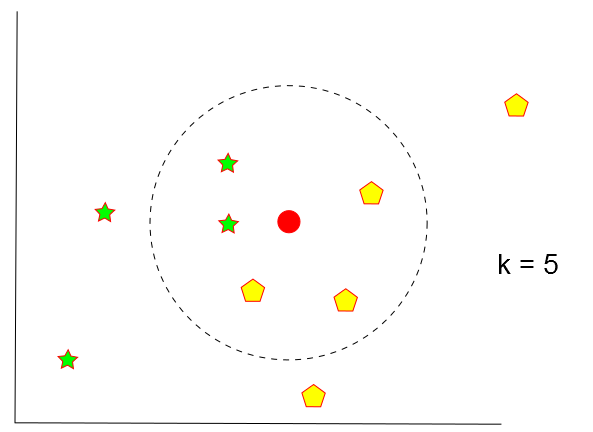
\includegraphics[keepaspectratio=true, scale=0.3]{neigh_small}
	\end{center}
	\item Odległo"sć od sąsiada okre"sla się na podstawie odpowiedniej metryki.
\end{itemize}
\end{frame}
\note{Czerwony punkt symbolizuje nowy obiekt \\
Etykiety wektorów ze zbioru uczącego to pięciokąt i gwiazdka \\
Dla $k = 5$ sąsiedztwo składa się z  2 gwiazdek i 3 pięciokątów. Stąd wniosek, że etykietą nowego obiektu będzie pięciokąt. \\
Sąsiedztwo okre"sla się przy pomocy odpowiedniej metryki. W tym przypadku jest to dystans euklidesowy.}

\begin{frame}{Różne rozmiary sąsiedztw}
\begin{center}
	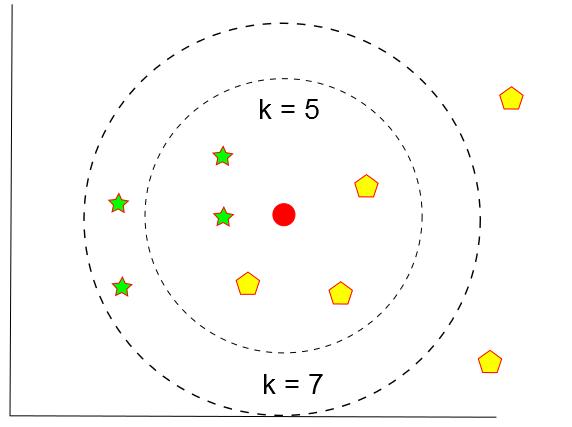
\includegraphics[keepaspectratio=true, scale=0.55]{neigh_k_small}
\end{center}
\end{frame}

\note{Rysunek ilustruje wpływ rozmiaru sąsiedztwa na klasyfikację. \\
Dla $k = 7$ w sąsiedztwie czerwonego punktu znajdują się dodatkowo 2 gwiazdki. \\
Powoduje to, że nowy obiekt otrzyma inną etykietę niż dla $k = 5$.}






\section{\scshape kNN - metryki}

\subsection{Własno"sci}
\begin{frame}{Własno"sci metryki ($D$)}
\begin{itemize}
	\item nieujemno"sć: $D(a,b) \ge 0$
	\item zwrotno"sć: $D(a,b) = 0 \Leftrightarrow a = b$
	\item symetria: $D(a,b) = D(b,a)$
	\item $D(a,b) + D(b,c) \ge D(a,c)$
\end{itemize}
\end{frame}

\subsection{Rodzaje metryk}
\begin{frame}{Metryka euklidesowa}
\begin{equation}
	\centering
	(a,b) = \sqrt{\sum_{i=1}^n{a_i - b_i}^2}
\end{equation}
\begin{itemize}
	\item Intuicyjna metryka (dystans między punktami).
	\item Wrażliwa na transformacje przestrzeni.
\end{itemize}
\end{frame}

\begin{frame}{Metryka Manhattan}
\begin{equation}
	\centering
	D(a,b) = \sum_{i=1}^n{|a_i - b_i|}
\end{equation}
\begin{itemize}
	\item Suma projekcji odcinków łączacych punkty na osie układu.
	\item Wrażliwa na rotację, ale nie translację.
\end{itemize}
\end{frame}

\begin{frame}{Metryka Hamminga}
\begin{itemize}
	\item Dwa ciągi znaków równej długo"sci.
	\item Liczba pozycji, na których znaki są różne
	\item {\color[rgb]{1,0,0} 5}{\color[rgb]{0,1,0} 	  23}{\color[rgb]{1,0,0} 4}{\color[rgb]{0,1,0} 1} \\
    {\color[rgb]{1,0,0} 4}{\color[rgb]{0,1,0} 23}{\color[rgb]{1,0,0} 5}{\color[rgb]{0,1,0} 1} \\
		  dystans = 2
\end{itemize}
\end{frame}

\begin{frame}{Metryka Tanimoto}
\begin{equation}
	\centering
	D(S_1,S_2) = \frac{n_1 + n_2 - 2n_12}{n_1 + n_2 - n_12}
\end{equation}
\begin{itemize}
	\item Użyteczna w taksonomii.
	\item Najlepiej działa dla takich samych lub zupełnie różnych zbiorów (bez gradacji).
\end{itemize}
\end{frame}
\section{\scshape kNN - dodatkowe}

\subsection{Złożono"sć}
\begin{frame}{Złożono"sć obliczeniowa}
\begin{itemize}
	\item Niski koszt fazy uczenia się.
	\item Wysoki koszt klasyfikacji.
	\item $O(dn)$
\end{itemize}
\end{frame}

\begin{frame}{Wielowymiarowo"sć}
\begin{itemize}
	\item Dobra wydajno"sć dla niewielkiej liczby wymiarów.
	\item Przy wielu wymiarach wszystkie punkty są od siebie odległe.
	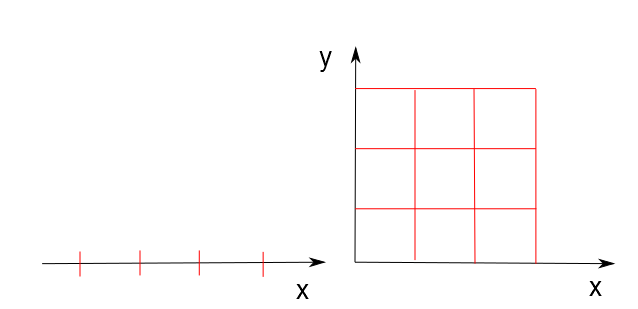
\includegraphics[keepaspectratio=true, scale=0.55]{dims_small}
\end{itemize}
\end{frame}


\subsection{Ważone kNN}
\begin{frame}{Ważone kNN}
\begin{itemize}
	\item Sąsiedzi położeni blisko mają większą wagę
	\item \textbf{Każdy} sąsiad bierze udział w etykietowaniu.
	\item Decyduje ważona większo"sć.
\end{itemize}
\end{frame}


\subsection{Zastosowanie}
\begin{frame}{Zastosowanie}
\begin{itemize}
	\item Sytuacje trudne do modelowania w klasyczny sposób.
	\item Zależno"sć między zmiennymi jest nietypowa.
	\item Metody klasyczne są bardziej użyteczne w przypadku niezłożono"sci relacji.
\end{itemize}
\end{frame}


\end{document}